\documentclass[12pt]{article}

\usepackage{amsmath}
\usepackage{amssymb}
\usepackage{graphicx}
\usepackage{algpseudocode}% http://ctan.org/pkg/algorithmicx
\usepackage{framed} % or, "mdframed"
%\usepackage{minipage}
\usepackage[framed]{ntheorem}
\usepackage{listings}
\usepackage{framed}
\usepackage{tikz}
\newcommand*\circled[1]{\tikz[baseline=(char.base)]{
            \node[shape=circle,draw,inner sep=2pt] (char) {#1};}}
\newframedtheorem{frm-thm}{Lemma}

\usepackage[scale=1.0, left=1.0cm, right=1.0cm, top=1.865cm, bottom=0.865cm]{geometry}
\DeclareMathOperator*{\argmin}{arg\,min}

\pagestyle{myheadings}
\markright{CSE 190 Final Exam \hfill Matthias Springer, A99500782\hfill}

\begin{document}

\section*{Problem 1: Using duality to prove optimality}
\subsection*{Basic Idea}
\begin{itemize}
	\item Let $D$ be the dual linear program of $P$, $x^*$ be a feasible solution for $P$, and $y^*$ be a feasible solution for $D$. According to the complementary slackness theorem, the following statements are equivalent.
	\begin{itemize}
		\item $x^*$ is optimal for $P$ and $y^*$ is optimal for $D$.
		\item For every constraint $i$ in $P$, $x^*$ satiesfies the $i$th constraint with equality, i.e. without slack, or $y_i^* = 0$ in $D$. For every constraint $j$ in $D$, $y^*$ satisfies the $j$th constraint with equality, or $x_j^* = 0$ in $P$.
	\end{itemize}
	\item $x^*$ satisfies the constraints $1$, $2$, $5$ with equality in $P$.
	\item $x_3^* \not= 0 \wedge x_4^* \not= 0 \wedge x_6^* \not= 0$, therefore we replace the 3rd, 4th, and 6th constraint in $D$ with equality constraints.
	\item We set $y_3^* = y_4^* = y_6^* = 0$ in $D$ and show that the the problem is still feasible. This proves that $x^*$ and $y^*$ are optimal.
\end{itemize}

\subsection*{Proof}
We check which constraints in $P$ are satisfied by $x^*$ with equality, i.e. without slack.
\begin{align*}
x_1 - 4 x_3 + 3 x_4 + x_5 + x_6 &= 1 & \text{no slack} \\
5 x_1 + 3 x_2 + x_3 - 5 x_5 + 3 x_6 &= 4 & \text{no slack} \\
4 x_1 + 5 x_2 - 3 x_3 + 3 x_4 - 4 x_5 + x_6 &= \frac{7}{2} < 4 & \text{slack} \\
-x_2 + 2 x_4 + x_5 - 5 x_6 &= \frac{9}{2} < 5 & \text{slack} \\
-2 x_1 + x_2 + x_3 + x_4 + 2 x_5 + 2 x_5 &=7 & \text{no slack} \\
2 x_1 - 3 x_2 + 2 x_3 - x_4 + 4 x_5 + 5 x_6 &= 4 < 5 & \text{slack}
\end{align*}
We write down the dual linear program $D$.
%\begin{figure}[h]
\begin{align*}
\text{minimize} \quad y_1 + 4 y_2 + 4 y_3 + 5 y+4 + 7 y_5 + 5 y_6& \\
\text{subject to} \quad  y_1 + 5 y_2 + 4 y_3 - y_4 - 2 y_5 + 2 y_6 &\geq 4 \\
3 y_2 + 5 y_2 - y_4 + y_5 - 3 y_6 &\geq 5 \\
-4 y_1 + y_2 - 3 y_3 + y_5 + 2 y_6 &\geq 1 \\
3 y_1 + 3 y_3 + 2 y_4 + y_5 - y_6 &\geq 3 \\
y_1 - 5 y_2 - 4 y_3 + y_4 + 2 y_5 + 4 y_6 &\geq -5\\
y_1 + 3 y_2 + y_3 -  y_4 + 2 y_5 + 5 y_6 & \geq 8 \\
y_1, y_2, y_3, y_4, y_5 &\geq 0
\end{align*}
%\caption{Dual linear program}
%\end{figure}
If $x^*$ is an optimal solution if $D$ has a feasible solution with $y_3 = y_4 = y_6 = 0$ and equality constraints $i$ for $x_i^* \not= 0$.
\begin{align*}
\text{minimize} \quad y_1 + 4 y_2 + 7 y_5 &\\
\text{subject to} \quad y_1 + 5 y_2 - 2 y_5 &\geq 4 \\
3 y_2 + y_5 &\geq 5 \\
-4 y_1 + y_2 + y_5 &= 1 \\
3 y_1 + y_5 &= 3 \\
y_1 - 5 y_2 + 2 y_5 &\geq -5 \\
y_1 + 3 y_2 + 2 y_5 &= 8 \\
y_1, y_2, y_5 &\geq 0
\end{align*}
This linear system contains three equations with three equalities. We can solve it and get $y_1= \frac{1}{2}$ and $y_2 = y_5 = \frac{3}{2}$. These values also satisfy the inequalities. Therefore, $x^*$ is an optimal solution. Also, if we plug in the values for $x^*$ and $y^*$ in the objective function for $P$ and $D$, we get the same value $17$.\hfill $\blacksquare$

\newpage
\section*{Problem 2: Simplex Method}
We transform the linear program to equational form.
\begin{align*}
\text{maximize} \quad 3 x_1 + x_2& \\
\text{subject to} \quad  x_1 - x_2 + x_3 &= -1 \\
-x_1 - x_2 - x_4 &= -3 \\
2 x_1 + x_2 + x_5 &= 4 \\
x_1, x_2, x_3, x_4, x_5 &\geq 0
\end{align*}

\subsection*{Auxiliary linear program (Simplex Phase 1)}
We solve an auxiliary linear program to find an initial basic feasible solution. We multiply the first and the second constraint with $-1$ and add a slack variable for every constraint.
\begin{align*}
\text{maximize} \quad -x_6 - x_7 - x_8 & \\
\text{subject to} \quad  -x_1 + x_2 - x_3 + x_6 &= 1 \\
x_1 + x_2 - x_4 + x_7 &= 3 \\
2 x_1 + x_2 + x_5 + x_8 &= 4 \\
x_1, x_2, x_3, x_4, x_5, x_6, x_7, x_8 &\geq 0
\end{align*}
We solve the auxiliary linear program with the simplex method. $x_6 = 1$, $x_7 = 3$, $x_8=4$, $x_1=x_2=x_3=x_4=x_5=0$ is an initial basic feasible solution.

\begin{framed}
\begin{minipage}[t]{0.5\textwidth}
\vspace{0.25cm}
\begin{tabular}{c | c}
$x_6 $ & $= 1 + x_1 - x_2 + x_3$ \\
$x_7 $ & $= 3 - x_1 - x_2 + x_4$ \\
$x_8 $ & $= 4 - 2x_1 - x_2 - x_5$ \\
\hline
$z $ & $=-8 + 2 x_1 + 3 x_2 - x_3 - x_4 + x_5$
\end{tabular}
\end{minipage}
\begin{minipage}[t]{0.5\textwidth}
\vspace{0.1cm}
\begin{itemize}
	\item Pivot by $x_2$
	\item \circled{$x_6$} $x_2 \leq 1$, \circled{$x_7$} $x_2 \leq 1$, \circled{$x_8$} $x_2 \leq 1$
	\item New non-basic variable: $x_6$
\end{itemize}
\vspace{0.0cm}
\end{minipage}
\end{framed}

\begin{framed}
\begin{minipage}[t]{0.5\textwidth}
\vspace{0.25cm}
\begin{tabular}{c | c}
$x_2 $ & $= 1 + x_1 + x_3 - x_6$ \\
$x_7 $ & $= 2 - 2x_1 - x_3 + x_6 + x_4$ \\
$x_8 $ & $= 3 - 3x_1 - x_3 - x_5 + x_6$ \\
\hline
$z $ & $= -5 + 5x_1 + 2x_3 - 3x_6 - x_4 + x_5$
\end{tabular}
\end{minipage}
\begin{minipage}[t]{0.5\textwidth}
\vspace{0.1cm}
\begin{itemize}
	\item Pivot by $x_3$
	\item \circled{$x_2$} unconstr., \circled{$x_7$} $x_3 \leq 2$, \circled{$x_8$} $x_3 \leq 3$
	\item New non-basic variable: $x_7$
\end{itemize}
\vspace{0.0cm}
\end{minipage}
\end{framed}

\begin{framed}
\begin{minipage}[t]{0.5\textwidth}
\vspace{0.25cm}
\begin{tabular}{c | c}
$x_3 $ & $= 2 - 2x_1 + x_4 + x_6 - x_7$ \\
$x_2 $ & $= 3 - x_1 + x_4 - x_7$ \\
$x_8 $ & $= 1 - x_1 - x_4 - x_5 + x_7$ \\
\hline
$z $ & $=-1 + x_1 + x_4 - x_6 - 2 x_7 + x_5$
\end{tabular}
\end{minipage}
\begin{minipage}[t]{0.5\textwidth}
\vspace{0.1cm}
\begin{itemize}
	\item Pivot by $x_5$
	\item \circled{$x_3$} unconstr., \circled{$x_2$} unconstr., \circled{$x_8$} $x_5 \leq 1$
	\item New non-basic variable: $x_8$
\end{itemize}
\vspace{0.0cm}
\end{minipage}
\end{framed}

\begin{framed}
\begin{minipage}[t]{0.5\textwidth}
\vspace{0.25cm}
\begin{tabular}{c | c}
$x_5 $ & $= 1 - x_1 - x_4 + x_7 - x_8$ \\
$x_3 $ & $= 2 - 2x_1 + x_4 + x_6 - x_7$ \\
$x_2 $ & $= 3 - x_1 + x_4 - x_7$ \\
\hline
$z $ & $=-x_6 - x_7 - x_8$
\end{tabular}
\end{minipage}
\begin{minipage}[t]{0.5\textwidth}
\vspace{0.1cm}
\begin{itemize}
	\item Optimal solution found
	\item Solution: $x_5 = 1$, $x_3 = 2$, $x_2 = 3$, others $0$
	\item Objective function value $0$, thus feasible
\end{itemize}
\vspace{0.0cm}
\end{minipage}
\end{framed}

\subsection*{Solve linear program (Simplex Phase 2)}
We use the solution from the auxiliary linear program as an initial basic feasible solution and run the simplex algorithm. In the auxiliary linear program, the objective function value was $0$, therefore, its solution was a basic feasible solution for the actual linear program.
\begin{framed}
\begin{minipage}[t]{0.5\textwidth}
\vspace{0.25cm}
\begin{tabular}{c | c}
$x_5 $ & $= 1 - x_1 + x_4$ \\
$x_3 $ & $= 2 - 2 x_1 - x_4$ \\
$x_2 $ & $= 3 - x_1 - x_4$ \\
\hline
$z $ & $= 3 + 2 x_1 - x_4$
\end{tabular}
\end{minipage}
\begin{minipage}[t]{0.5\textwidth}
\vspace{0.1cm}
\begin{itemize}
	\item Pivot by $x_1$
	\item \circled{$x_5$} $x_1 \leq 1$, \circled{$x_3$} $x_1 \leq 1$, \circled{$x_2$} $x_1 \leq 3$
	\item New non-basic variable: $x_5$
\end{itemize}
\vspace{0.0cm}
\end{minipage}
\end{framed}

\begin{framed}
\begin{minipage}[t]{0.5\textwidth}
\vspace{0.25cm}
\begin{tabular}{c | c}
$x_1 $ & $= 1 + x_4 - x_5$ \\
$x_3 $ & $= -3 x_4 + 2 x_5$ \\
$x_2 $ & $= 2 - 2 x_4 + x_5$ \\
\hline
$z $ & $= 5 + x_4 - 2 x_5$
\end{tabular}
\end{minipage}
\begin{minipage}[t]{0.5\textwidth}
\vspace{0.1cm}
\begin{itemize}
	\item Pivot by $x_4$
	\item \circled{$x_1$} unconstr., \circled{$x_3$} $x_4 \leq 0$, \circled{$x_2$} $x_4 \leq 1$
	\item New non-basic variable: $x_3$
\end{itemize}
\vspace{0.0cm}
\end{minipage}
\end{framed}

\begin{framed}
\begin{minipage}[t]{0.5\textwidth}
\vspace{0.25cm}
\begin{tabular}{c | c}
$x_4 $ & $= \frac{2 x_5}{3} - \frac{x_3}{3}$ \\
$x_1 $ & $= 1 - \frac{x_5}{3} - \frac{x_3}{3}$ \\
$x_2 $ & $= 2 - \frac{x_5}{3} + \frac{2 x_3}{3}$ \\
\hline
$z $ & $= 5 - \frac{x_3}{3} - 2 x_5$
\end{tabular}
\end{minipage}
\begin{minipage}[t]{0.5\textwidth}
\vspace{0.1cm}
\begin{itemize}
	\item Optimal solution found
	\item Solution: $x_1 = 1$, $x_2 = 2$, $x_3 = x_4 = x_5 = 0$
\end{itemize}
\vspace{0.0cm}
\end{minipage}
\end{framed}
\noindent $x_1 = 1$, $x_2=2$, $x_3 = 0$ is an optimal solution for the linear program, achieving an objective function value $5$.

\newpage
\section*{Problem 3: Formulating the dual program}
\begin{minipage}[t]{0.5\textwidth}
\begin{align*}
\text{maximize} \quad x_1 + x_2 + x_3 & \\
\text{subject to} \quad  x_1 + x_3 &\leq 2 \\
x_1 + 2 x_2 &= 2 \\
x_1 + x_2 + x_3 &\leq 3 \\
x_1, x_3 &\leq 0
\end{align*}
\end{minipage}
\begin{minipage}[t]{0.5\textwidth}
\begin{align*}
\text{minimize} \quad 2y_1 + 2y_2 + 3y_3 & \\
\text{subject to} \quad  y_1 + y_2 + y_3 &\leq 1 \\
2y_2 + y_3 &= 1 \\
y_1 + y_3 &\leq 1 \\
y_1, y_3 &\geq 0
\end{align*}
\end{minipage}

\newpage
\section*{Problem 4}
$A_x$ and $B_x$ are variables for the amount of raw gasoline of type $x$ in Avgas A and Avgas B, respectively. $A$ and $B$ is the amount of produced Avgas A and Avgas B. $R_x$ is the amount of sold raw gasoline of type $x$. $R$ is the total amount of sold raw gasoline.

\begin{align*}
\text{maximize} \quad 6.45 A + 5.91 B + 4.83 R & \\
\text{subject to} \quad 107 A_A + 93 A_C + 87 A_S + 108 A_I &\geq 100 A \\
107 B_A + 93 B_C + 87 B_S + 1087 B_I &\geq 91 B \\
5 A_A + 8 A_C + 4 A_S + 21 A_I &\leq 7 A \\
5 B_A + 8 B_C + 4 B_S + 21 B_I &\leq 7 B \\
A_A + A_C + A_S + A_I &= A \\
B_A + B_C + B_S + B_I &= B \\
R_A + R_C + R_S + R_I &= R \\
R_A + A_A + B_A &= 3814 \\
R_C + A_C + B_C &= 2666 \\
R_S + A_S + B_S &= 4016 \\
R_I + A_I + B_I &= 1300 \\
A, A_A, A_C, A_S, A_I, B, B_A, B_C, B_S, B_I, R, R_A, R_C, R_S, R_I &\geq 0
\end{align*}
Now, we convert the linear program to canonical form.
\begin{align*}
\text{maximize} \quad 6.45 A + 5.91 B + 4.83 R & \\
\text{subject to} \quad -107 A_A - 93 A_C - 87 A_S - 108 A_I + 100 A &\leq 0 \\
-107 B_A - 93 B_C - 87 B_S - 1087 B_I + 91 B &\leq 0 \\
5 A_A + 8 A_C + 4 A_S + 21 A_I - 7A &\leq 0 \\
5 B_A + 8 B_C + 4 B_S + 21 B_I - 7B &\leq 0 \\
A_A + A_C + A_S + A_I - A &\leq 0 \\
-A_A - A_C - A_S - A_I + A &\leq 0 \\
B_A + B_C + B_S + B_I - B &\leq 0 \\
-B_A - B_C - B_S - B_I + B &\leq 0 \\
R_A + R_C + R_S + R_I - R &\leq 0 \\
-R_A - R_C - R_S - R_I + R &\leq 0 \\
R_A + A_A + B_A &\leq 3814 \\
-R_A - A_A - B_A &\leq -3814 \\
R_C + A_C + B_C &\leq 2666 \\
-R_C - A_C - B_C &\leq -2666 \\
R_S + A_S + B_S &\leq 4016 \\
-R_S - A_S - B_S &\leq -4016 \\
R_I + A_I + B_I &\leq 1300 \\
-R_I - A_I - B_I &\leq -1300 \\
A, A_A, A_C, A_S, A_I, B, B_A, B_C, B_S, B_I, R, R_A, R_C, R_S, R_I &\geq 0
\end{align*}

\newpage
\section*{Problem 5: Nash equilibrium}
\begin{minipage}[t]{0.5\textwidth}
\textbf{Row Player}
\begin{align*}
\text{maximize} \quad x_0 & \\
\text{subject to} \quad  -x_1 - x_2 - x_0 &\geq 0 \\
x_1 - x_2 + x_3 - x_0 &\geq 0 \\
-x_1 + x_2 + x_3 - x_0 &\geq 0 \\
2 x_1 + x_2 - x_3 - x_0 &\geq 0 \\
x_1 + x_2 + x_3  &= 1 \\
x_1, x_2, x_3 &\geq 0
\end{align*}
\end{minipage}
\begin{minipage}[t]{0.5\textwidth}
\textbf{Column Player}
\begin{align*}
\text{minimize} \quad y_0 & \\
\text{subject to} \quad  -y_1 + y_2 - y_3 + 2 y_4 - y_0 &\leq 0 \\
-y_1 - y_2 + y_3 + y_4 - y_0 &\leq 0 \\
y_2 + y_3 - y_4 - y_0 &\leq 0 \\
y_1 + y_2 + y_3 + y_4 &= 1\\
y_1, y_2, y_3, y_4 &\geq 0
\end{align*}
\end{minipage}

\subsection*{Solving with the Simplex Method (Row Player)}
We transform the linear program to equational form by introducing new slack variables and substituting $x_0 = x_4 - x_5$, where $x_4, x_5 \geq 0$.
\begin{align*}
\text{maximize} \quad x_4 - x_5 & \\
\text{subject to} \quad -x_1 - x_2 - x_4 + x_5 - x_6 &= 0 \\
x_1 - x_2 + x_3 - x_4 + x_5 - x_7 &= 0 \\
-x_1 + x_2 + x_3 - x_4 + x_5 - x_8 &= 0 \\
2 x_1 - x_2 - x_3 - x_4 + x_5 - x_9 &= 0 \\
x_1 + x_2 + x_3 &= 1\\
x_1, x_2, x_3, x_4, x_5, x_6, x_7, x_8, x_9 &\geq 0
\end{align*}
Using trail and error, we guess an initial basic feasible solution: $x_1 = x_2 = x_4 = x_9 = 0$, $x_3 = 1$, $x_5 = 1$, $x_8 = 2$, $x_7 = 2$, $x_6 = 1$. We use the simplex method to solve the linear program.

\begin{framed}
\begin{minipage}[t]{0.5\textwidth}
\vspace{0.25cm}
\begin{tabular}{c | c}
$x_3$ & $= 1 - x_2 - x_1$ \\
$x_6$ & $= 1 - 4 x_1 - x_2 + x_9$ \\
$x_7$ & $= 2 - 2x_2 - 3x_1 + x_9$ \\
$x_8$ & $= 2 - 3x_1 + x_9$ \\
$x_5$ & $= 1 - 3x_1 + x_4 + x_9$ \\
\hline
$z $ & $= -1 + 3x_1 - x_9$
\end{tabular}
\end{minipage}
\begin{minipage}[t]{0.5\textwidth}
\vspace{0.1cm}
\begin{itemize}
	\item Pivot by $x_1$
	\item \circled{$x_3$} $x_1 \leq 1$, \circled{$x_6$} $x_1 \leq \frac{1}{4}$ 
	\item \circled{$x_7$} $x_1 \leq \frac{2}{3}$, \circled{$x_8$} $x_1 \leq \frac{2}{3}$, \circled{$x_5$} $x_1 \leq \frac{1}{3}$
	\item New non-basic variable: $x_6$
\end{itemize}
\vspace{0.0cm}
\end{minipage}
\end{framed}

\begin{framed}
\begin{minipage}[t]{0.5\textwidth}
\vspace{0.25cm}
\begin{tabular}{c | c}
$x_1$ & $= \frac{1}{4} - \frac{x_2}{4} + \frac{x_9}{4} - \frac{x_6}{4}$ \\
$x_3$ & $= \frac{3}{4} - \frac{3x_2}{4} - \frac{x_9}{4} + \frac{x_6}{4}$ \\
$x_7$ & $= \frac{5}{4} - \frac{5x_2}{4} + \frac{x_9}{4} + \frac{3x_6}{4}$ \\
$x_8$ & $= \frac{5}{4} + \frac{3x_2}{4} + \frac{x_9}{4} + \frac{3 x_6}{4}$ \\
$x_5$ & $= -\frac{1}{4} - \frac{3x_2}{4} - \frac{x_9}{4} + \frac{3 x_6}{4} + x_4$ \\
\hline
$z $ & $= -\frac{1}{4} - \frac{3 x_2}{4} - \frac{x_9}{4} - \frac{3 x_6}{4}$
\end{tabular}
\end{minipage}
\begin{minipage}[t]{0.5\textwidth}
\vspace{0.1cm}
\begin{itemize}
	\item Optimal solution found
	\item $x_0 = x_4 - x_5 = -\frac{1}{4}$ 
	\item $x_1 = \frac{1}{4}$, $x_2 = 0$, $x_3 = \frac{3}{4}$
\end{itemize}
\vspace{0.0cm}
\end{minipage}
\end{framed}

\subsection*{Solving with the Simplex Method (Column Player)}
We transform the linear program to equational form by introducing new slack variables and substituting $y_0 = y_6 - y_5$, where $y_6, y_5 \geq 0$.
\begin{align*}
\text{maximize} \quad y_5 - y_6 & \\
\text{subject to} \quad -y_1 + y_2 - y_3 + 2 y_4 + y_5 - y_6 + y_7 &= 0 \\
-y_1 - y_2 + y_3 + y_4 + y_5 - y_6 - y_8 &= 0 \\
y_2 + y_3 - y_4 + y_5 - y_6 + y_9 &= 0 \\
y_1 + y_2 + y_3 + y_4 &= 1 \\
y_1, y_2, y_3, y_4, y_5, y_6, y_7, y_8, y_9 &\geq 0
\end{align*}
Using trail and error, we guess an initial basic feasible solution: $y_2 = y_3 = y_4 = y_5 = y_6 = y_9 = 0$, $y_1 = 1$, $y_8 = 1$, $y_7 = 1$. We use the simplex method to solve the linear program.

\begin{framed}
\begin{minipage}[t]{0.5\textwidth}
\vspace{0.25cm}
\begin{tabular}{c | c}
$y_1$ & $= 1 - y_2 - y_3 - y_4$ \\
$y_6$ & $= y_2 + y_3 - y_4 + y_5 + y_9$ \\
$y_8$ & $= 1 + y_2 - y_3 - 3y_4 + y_9$ \\
$y_7$ & $= 1 - y_2 + y_3 - 4y_4 + y_9$ \\
\hline
$z $ & $= -y_2 - y_3 + y_4 - y_9$
\end{tabular}
\end{minipage}
\begin{minipage}[t]{0.5\textwidth}
\vspace{0.1cm}
\begin{itemize}
	\item Pivot by $y_4$
	\item \circled{$y_1$} $y_4 \leq 1$, \circled{$y_6$} $y_4 \leq 0$ 
	\item \circled{$y_8$} $y_4 \leq \frac{1}{3}$, \circled{$y_7$} $y_4 \leq 1$
	\item New non-basic variable: $y_6$
\end{itemize}
\vspace{0.0cm}
\end{minipage}
\end{framed}

\begin{framed}
\begin{minipage}[t]{0.5\textwidth}
\vspace{0.25cm}
\begin{tabular}{c | c}
$y_4$ & $= y_2 + y_3 + y_5 - y_6 + y_9$ \\
$y_1$ & $= 1 - 2y_2 - 2y_3 - y_5 + y_6 - y_9$ \\
$y_8$ & $= 1 - 2y_2 - 4y_3 - 3y_5 - 3y_6 - 3y_9$ \\
$y_7$ & $= 1 - 5y_2 - 3y_3 - 4y_5 - 4y_6 - 4y_9$ \\
\hline
$z $ & $= y_5 - y_6$
\end{tabular}
\end{minipage}
\begin{minipage}[t]{0.5\textwidth}
\vspace{0.1cm}
\begin{itemize}
	\item Pivot by $y_5$
	\item \circled{$y_4$} unconstr., \circled{$y_1$} $y_5 \leq 1$ 
	\item \circled{$y_8$} $y_5 \leq \frac{1}{3}$, \circled{$y_7$} $y_5 \leq \frac{1}{4}$
	\item New non-basic variable: $y_7$
\end{itemize}
\vspace{0.0cm}
\end{minipage}
\end{framed}

\begin{framed}
\begin{minipage}[t]{0.5\textwidth}
\vspace{0.25cm}
\begin{tabular}{c | c}
$y_4$ & $= \frac{1}{4} - \frac{y_2}{4} + \frac{y_3}{4} - y_6 - \frac{y_7}{4} - y_9$ \\
$y_1$ & $= \frac{3}{4} - \frac{3 y_2}{4} - \frac{5 y_3}{4} + y_6 + y_9 + \frac{y_7}{4}$ \\
$y_8$ & $= \frac{1}{4} + \frac{7 y_2}{4} + \frac{y_3}{4} + 3 y_6 + 3 y_9 + \frac{3 y_7}{4}$ \\
$y_5$ & $= \frac{1}{4} - \frac{5 y_2}{4} - \frac{3 y_3}{4} - y_6 - y_9 - \frac{y_7}{4}$ \\
\hline
$z $ & $= \frac{1}{4} - \frac{5 y_2}{4} - \frac{3 y_3}{4} - y_6 - y_9 - \frac{y_7}{4}$
\end{tabular}
\end{minipage}
\begin{minipage}[t]{0.5\textwidth}
\vspace{0.1cm}
\begin{itemize}
	\item Optimal solution found
	\item $y_0 = y_6 - y_5 = -\frac{1}{4}$
	\item $y_1 = \frac{3}{4}$, $y_2 = y_3 = 0$, $y_4 = \frac{1}{4}$
\end{itemize}
\vspace{0.0cm}
\end{minipage}
\end{framed}


\newpage
\section*{Problem 6: Flow Problem}
\subsection*{Linear Program}
\begin{align*}
\text{maximize} \quad f_{CT} + f_{DT} & \\
\text{subject to} \quad  0 \leq f_{SA} \leq 8 \\
0 \leq f_{SB} \leq 10 \\
0 \leq f_{AB} \leq 9 \\
0 \leq f_{AC} \leq 3 \\
0 \leq f_{BD} \leq 6 \\
0 \leq f_{AD} \leq 8 \\
0 \leq f_{BC} \leq 6 \\
0 \leq f_{CD} \leq 5 \\
0 \leq f_{CT} \leq 10 \\
0 \leq f_{DT} \leq 9 \\
f_{SA}  = f_{AB} + f_{AD} + f_{AC} \\
f_{SB} + f_{AB} = f_{BC} + f_{BD} \\
f_{AC} + f_{BC} = f_{CT} + f_{CD} \\
f_{BD} + f_{AD} + f_{CD} = f_{DT}
\end{align*}

\subsection*{AMPL Program}
\begin{lstlisting}
var fSA >= 0, <= 8;
var fSB >= 0, <= 10;
var fAB >= 0, <= 9;
var fAC >= 0, <= 3;
var fBD >= 0, <= 6;
var fAD >= 0, <= 8;
var fBC >= 0, <= 6;
var fCD >= 0, <= 5;
var fCT >= 0, <= 10;
var fDT >= 0, <= 9;

maximize flow: fCT + fDT;

subject to conservationA: fSA = fAB + fAD + fAC;
subject to conservationB: fSB + fAB = fBC + fBD;
subject to conservationC: fAC + fBC = fCT + fCD;
subject to conservationD: fBD + fAD + fCD = fDT;
\end{lstlisting}

\begin{framed}
\noindent AMPL outputs the following solution with an objective function value of $18$.

\vspace{0.5cm}
\noindent \begin{tabular}{c|cccccccccc}
Edge & $f_{SA}$ & $f_{SB}$ & $f_{AB}$ & $f_{AC}$ & $f_{BD}$ & $f_{AD}$ & $f_{BC}$ & $f_{CD}$ & $f_{CT}$ & $f_{DT}$ \\
\hline
Flow & 8 & 10 & 2 & 3 & 6 & 3 & 6 & 0 & 9 & 9 
\end{tabular}
\end{framed}

\subsection*{Max-flow and Min-cut}
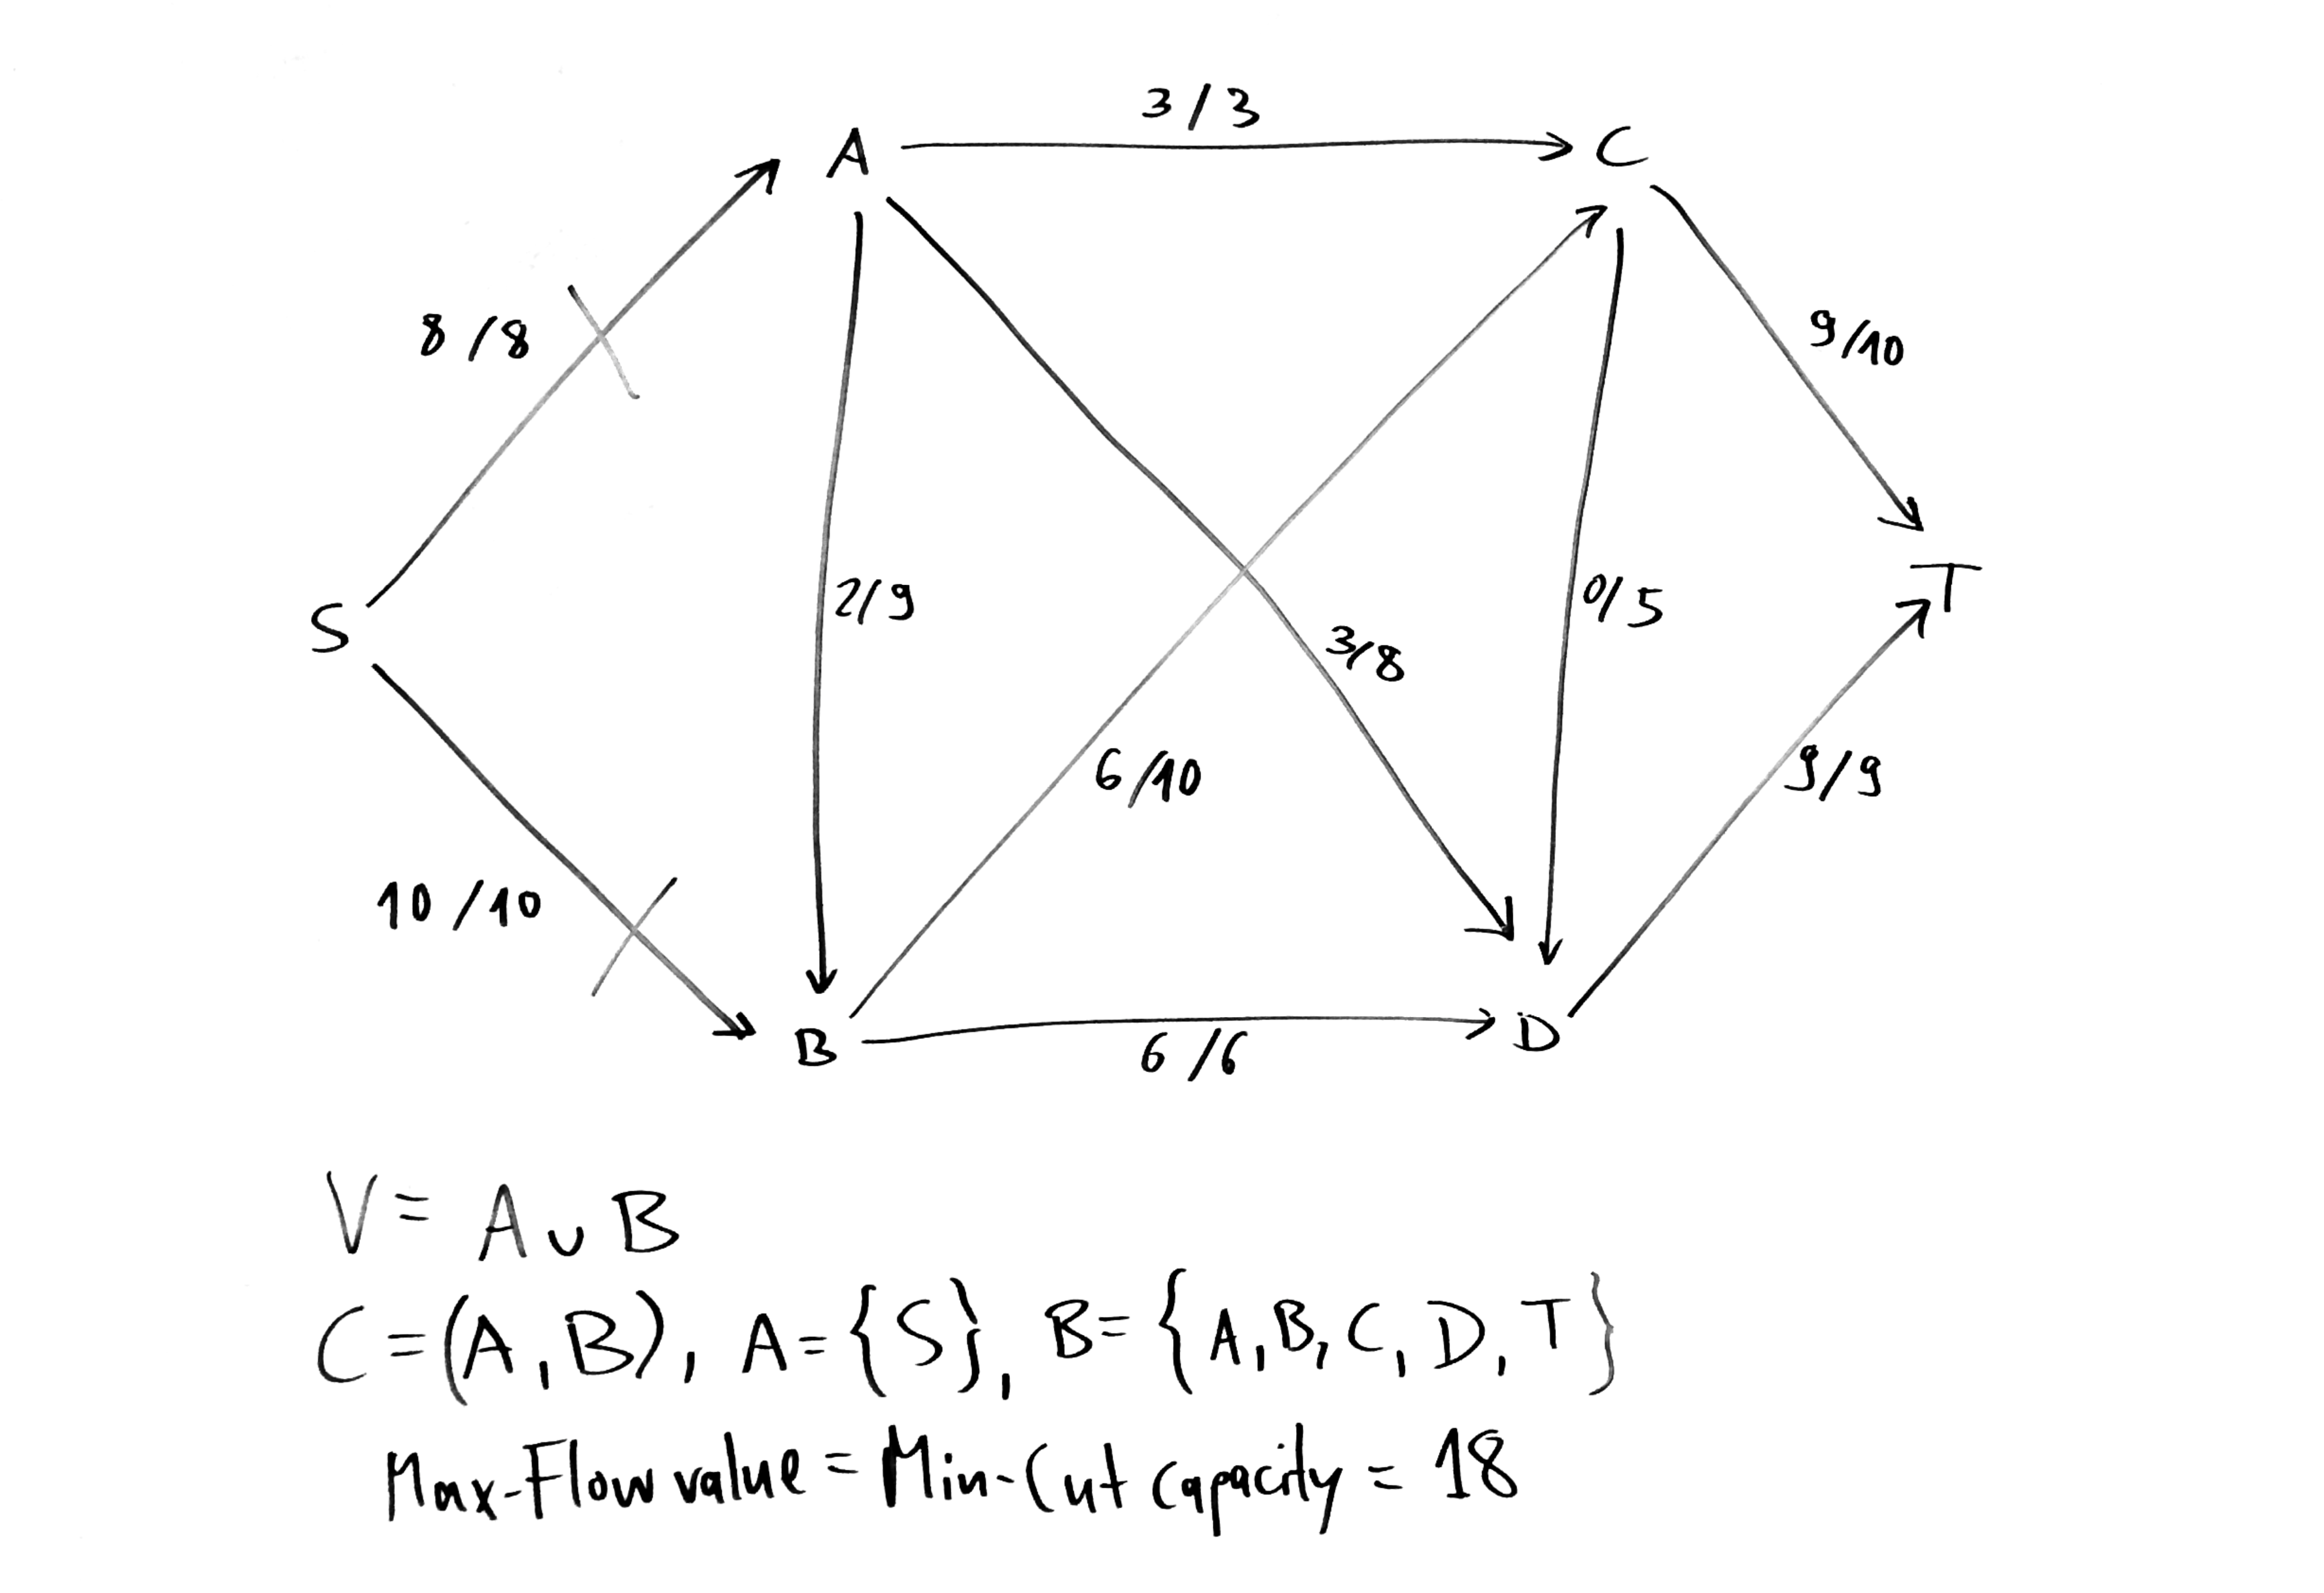
\includegraphics[width=\textwidth]{6_1.pdf}
The minimum cut cuts the edges $SA$ and $SB$, resulting in two vertex sets $\{S\}$ and $V-\{S\}$.
\end{document}

